\documentclass[10pt,a4paper]{article}
\usepackage[utf8]{inputenc}
\usepackage[T1]{fontenc}
\usepackage{amsmath}
\usepackage{amssymb}
\usepackage{graphicx}
\usepackage{multirow, multicol}
\usepackage{booktabs}
\graphicspath{{images/}}

\title{Data Mining; Assignemt 6}
\author{Jesse Annan \hspace{0.5cm} | \hspace{0.5cm} ID: 002708111}
\begin{document}
	\maketitle
	
	\clearpage
	
	\textbf{Find step by step procedure of 1-5 in attached excel file.}
	\begin{enumerate}
		\item K-means algorithm \newline
			Starting with k=4 clusters. I selected \textit{(0,7), (4,4), (0,0), \textrm{and} (9,9)} as my initial cluster centers. \newline
			\text{d(x,y)} = Manhattan distance. \newline
			
			First Iteration:
			\begin{table}[h!]
				\centering
				\begin{tabular}{cccc}
					\toprule
					\multicolumn{4}{c}{Cluster centers} \\
					(0, 7) & (4, 4) & (0, 0) & (9, 9) \\
					cluster 1 &	cluster 2 &	cluster 3 & cluster 4 \\ \midrule
					(0,7) &	(2,5) &	(1,1) & (7,8) \\
					(1,6) &	(3,6) &	(3,0) &	(9,9) \\
					(1,8) &	(5,3) & & \\		
					(2,7) &	(6,2) & & \\		
					(2,8) & (6,4) & & \\		
					(3,7) & (7,2) & & \\		
					& (7,3) & & \\		
					& (7,5) & & \\	
					& (8,3) & & \\
					& (8,4) & & \\
					\bottomrule					
				\end{tabular}
			\end{table}
		
			Second Iteration:
			\begin{table}[h!]
				\centering
				\begin{tabular}{cccc}
					\toprule
					\multicolumn{4}{c}{Cluster centers} \\
					(1.5, 7.1$\dot{6}$) & (5.9, 3.7) & (2, 0.5) & (8, 8.5) \\
					cluster 1 &	cluster 2 &	cluster 3 & cluster 4 \\ \midrule
					(0,7) &	(5,3) &	(1,1) & (7,8) \\
					(1,6) &	(6,2) &	(3,0) &	(9,9) \\
					(1,8) &	(6,4) & & \\		
					(2,5) &	(7,2) & & \\		
					(2,7) & (7,3) & & \\		
					(2,8) & (7,5) & & \\		
				    (3,6) & (8,3) & & \\		
					(3,7) & (8,4) & & \\	
%					&  & & \\
%					&  & & \\
					\bottomrule					
				\end{tabular}
			\end{table}
		
			\clearpage
			Third Iteration:
			\begin{table}[h!]
				\centering
				\begin{tabular}{cccc}
					\toprule
					\multicolumn{4}{c}{Cluster centers} \\
					(1.75, 6.75) & (6.75, 3.25) & (2, 0.5) & (8, 8.5) \\
					cluster 1 &	cluster 2 &	cluster 3 & cluster 4 \\ \midrule
					(0,7) &	(5,3) &	(1,1) & (7,8) \\
					(1,6) &	(6,2) &	(3,0) &	(9,9) \\
					(1,8) &	(6,4) & & \\		
					(2,5) &	(7,2) & & \\		
					(2,7) & (7,3) & & \\		
					(2,8) & (7,5) & & \\		
					(3,6) & (8,3) & & \\		
					(3,7) & (8,4) & & \\	
					%					&  & & \\
					%					&  & & \\
					\bottomrule					
				\end{tabular}
			\end{table}
			
			Algorithm terminated since the clusters where the same.
			
		
		\clearpage
		\item K-medoid algorithm \newline
			Starting with k=4 clusters. I selected \textit{(1,8), (1,1), (2,5), \textrm{and} (7,8)} as my initial cluster centers. \newline
			\text{d(x,y)} = Manhattan distance. \newline
			
			First Iteration:
			\begin{table}[h!]
				\centering
				\begin{tabular}{cccc}
					\toprule
					\multicolumn{4}{c}{Cluster centers} \\
					(1, 8) & (1, 1) & (2, 5) & (7, 8) \\
					cluster 1 &	cluster 2 &	cluster 3 & cluster 4 \\ \midrule
					(0,7) & (1,1) & (1,6) & (7,2) \\
					(1,8) & (3,0) & (2,5) & (7,3) \\
					(2,7) & (6,2) & (3,6) & (7,5) \\
					(2,8) &  & (5,3) & (7,8) \\
					(3,7) &  & (6,4) & (8,3) \\
					 &  &  & (8,4) \\
					 &  &  & (9,9) \\ \midrule
					 \textit{Cost = 59}	& & & \\			
					\bottomrule					
				\end{tabular}
			\end{table}
		
			Second Iteration:
			\begin{table}[h!]
				\centering
				\begin{tabular}{cccc}
					\toprule
					\multicolumn{4}{c}{Cluster centers} \\
					(1, 8) & (1, 1) & (5, 3) & (7, 8) \\
					cluster 1 &	cluster 2 &	cluster 3 & cluster 4 \\ \midrule
					(0,7) & (1,1) & (5,3) & (7,5) \\
					(1,6) & (3,0) & (6,2) & (7,8) \\
					(1,8) &  & (6,4) & (9,9) \\
					(2,5) &  & (7,2) & \\
					(2,7) &  & (7,3) & \\
					(2,8) &  & (8,3) & \\
					(3,6) &  & (8,4) & \\ 
					(3,7) &  & 	& \\ \midrule
					\textit{Cost = 43} & & & \\	
					\bottomrule					
				\end{tabular}
			\end{table}
		
			\clearpage
			Third Iteration:
			\begin{table}[h!]
				\centering
				\begin{tabular}{cccc}
					\toprule
					\multicolumn{4}{c}{Cluster centers} \\
					(1, 8) & (1, 1) & (7, 3) & (7, 8) \\
					cluster 1 &	cluster 2 &	cluster 3 & cluster 4 \\ \midrule
					(0,7) & (1,1) & (5,3) & (7,8) \\
					(1,6) & (3,0) & (6,2) & (9,9) \\
					(1,8) &  & (6,4) & \\
					(2,5) &  & (7,2) & \\
					(2,7) &  & (7,3) & \\
					(2,8) &  & (7,5) & \\
					(3,6) &  & (8,3) & \\ 
					(3,7) &  & (8,4) & \\ \midrule
					\textit{Cost = 36} & & & \\		
					\bottomrule					
				\end{tabular}
			\end{table}
		
			Forth Iteration:
			\begin{table}[h!]
				\centering
				\begin{tabular}{cccc}
					\toprule
					\multicolumn{4}{c}{Cluster centers} \\
					(1, 8) & (1, 1) & (7, 3) & (7, 8) \\
					cluster 1 &	cluster 2 &	cluster 3 & cluster 4 \\ \midrule
					(0,7) & (1,1) & (5,3) & (7,8) \\
					(1,6) & (3,0) & (6,2) & (9,9) \\
					(1,8) &  & (6,4) & \\
					(2,5) &  & (7,2) & \\
					(2,7) &  & (7,3) & \\
					(2,8) &  & (7,5) & \\
					(3,6) &  & (8,3) & \\ 
					(3,7) &  & (8,4) & \\ \midrule
					\textit{Cost = 30} & & & \\		
					\bottomrule					
				\end{tabular}
			\end{table}
			
			Algorithm terminated because of the reduced cost and unchanged clusters.
			
			
		\clearpage
		\item AGNES algorithm \newline
			\text{d(x,y)} = Manhattan distance. \newline
			\begin{figure}[h!]
				\centering
				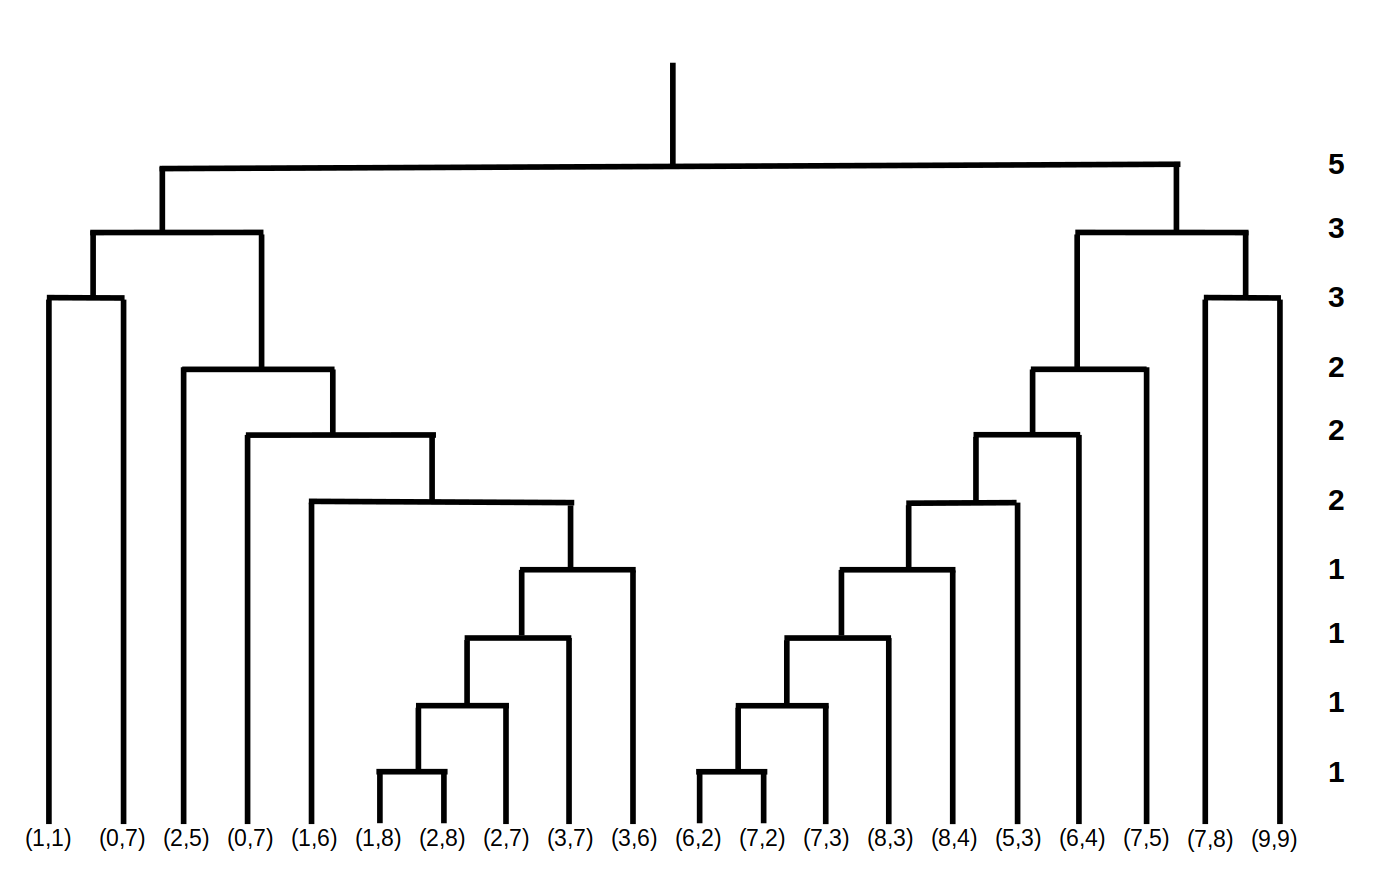
\includegraphics[scale=0.27]{agnes.png}
			\end{figure}
		
			Algorithm terminated because every single cluster joined the hierarchical tree.
		
		
		\clearpage
		\item DBSCAN algorithm \newline
			\text{d(x,y)} = Euclidean distance. \newline
			\begin{table}[h!]
				\centering
				\begin{tabular}{cccccc}
					\toprule
					\multicolumn{6}{c}{Core points} \\ \midrule
					(1,6) & (1,8) & (2,7) & (2,8) & (3,6) & (3,7) \\
					(6,2) & (6,4) & (7,2) & (7,3) & (8,3) & (8,4) \\ \hline \hline
					\multicolumn{6}{c}{Border points} \\ \midrule
					& (0,7) & (2,5) & (5,3) & (7,5) & \\
					\bottomrule
				\end{tabular}
			\end{table}
			
			Clustering core points.
			
			\begin{table}[h!]
				\centering
				\begin{tabular}{c|cccccc}
					\toprule
					\multicolumn{7}{c}{Core points} \\ \midrule
					Cluster 1 & (1,6) & (1,8) & (2,7) & (2,8) & (3,6) & (3,7) \\
					Cluster 2 & (6,2) & (6,4) & (7,2) & (7,3) & (8,3) & (8,4) \\ 
					\bottomrule
				\end{tabular}
			\end{table}
		
			Adding border points to the clusters
			
			\begin{table}[h!]
				\centering
				\begin{tabular}{c|cccccccc}
					\toprule
					\multicolumn{9}{c}{Cluster points} \\ \midrule
					Cluster 1 & (0,7) & (1,6) & (1,8) & (2,5) & (2,7) & (2,8) & (3,6) & (3,7) \\
					Cluster 2 & (5,3) & (6,2) & (6,4) & (7,2) & (7,3) & (7,5) & (8,3) & (8,4) \\
					\hline \hline
					\multicolumn{9}{c}{Outlier points} \\ \midrule
					\multicolumn{2}{c}{} & (1,1) & (3,0) & (7,8) & (9,9) & & & \\ 
					\bottomrule
				\end{tabular}
			\end{table}
			
			
		
		\clearpage
		\item OPTICS algorithm \newline
			\text{d(x,y)} = Manhattan distance. \newline
			\begin{figure}[h!]
				\centering
				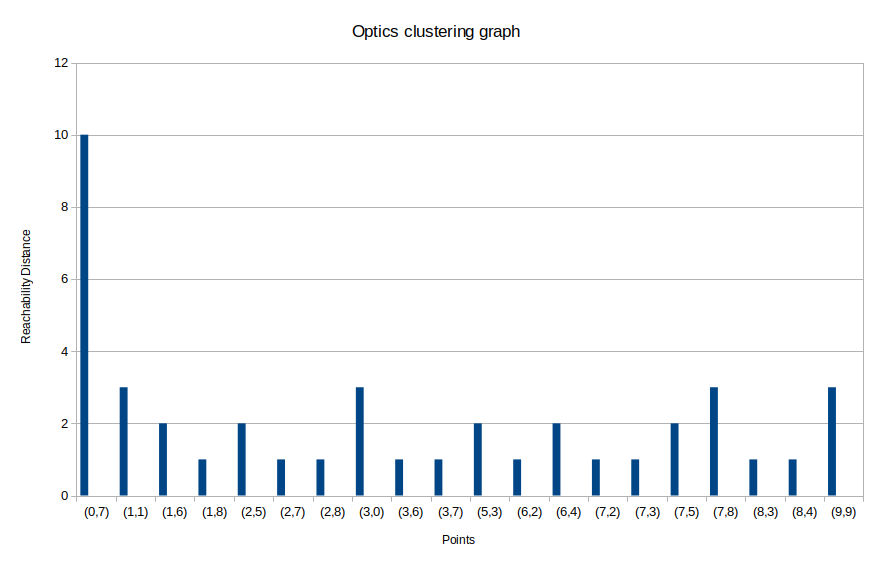
\includegraphics[scale=0.45]{optics.png}
			\end{figure}
		
		
		\clearpage
		\item Spectral clustering algorithm \newline
			\textit{Kindly check attached jupyter notebook file.}
			
			
			
	\end{enumerate}
	
\end{document}